%!Tex Program = xelatex
\documentclass[a4paper]{ctexart} % 使用 ctexart 支持中文
\usepackage{amsmath} % 数学公式支持
\usepackage{amsfonts} % 数学符号支持
\usepackage{amssymb} % 数学符号支持
\usepackage{graphicx} % 图片支持
\usepackage{subcaption} % 子图支持
\usepackage{fontspec} % 字体支持

% 定义拉普拉斯算子
\newcommand{\laplace}{\ensuremath{\Delta}}

% 文档信息
\title{Project2 Report}
\author{王方宸 \\ 学号：3210105371}
\date{2024年4月8日}

\begin{document}
\maketitle

\pagestyle{empty}

\section{问题描述}
本项目的目标是在给定区域 $\Omega$ 上使用有限差分方法，求解泊松方程 $-\laplace u = f$，其中区域 $\Omega$ 和边界条件由用户指定，由Multigrid对线性系统进行求解。具体问题描述如下：

\subsection{区域定义}
\begin{itemize}
    \item[(a)] 一维区域 $\Omega = (0, 1)$；
    \item[(b)] 正方形区域 $\Omega = (0, 1)^2$；
\end{itemize}

\subsection{边界条件}
用户可以选择以下边界条件之一：
\begin{itemize}
    \item Dirichlet 边界条件；
    \item Neumann 边界条件；
    \item 混合边界条件（部分 Dirichlet，部分 Neumann）。
\end{itemize}

\section{离散实现与理论分析}
\subsection{格点离散}
本次的离散基本上是对之前$project1$的延续,内部格点使用的是五点差分格式,但是对neumann边界不使用$ghost cell$,而是采用讲义使用内部三个点的插值格式:

\[-\frac{1}{\hbar}\left(\frac{3}{2}U_{0}-2U_{1}+\frac{1}{2}U_{2}\right)=\sigma+O(\hbar^{2}).\] 
\subsection{限制和延伸算子操作}
对一维的算子完全按照讲义方法，只有二次插值自行处理。为了得到对称的格式，对内部格点，在粗网格位置 $ih + h/2$ 处的点，分别用：

\begin{itemize}
    \item 第一组：$(ih, (i+1)h, (i+2)h)$
    \item 第二组：$((i-1)h, ih, (i+1)h)$
\end{itemize}

分别做二次插值后取平均，得到对称格式：

\[
U_{2i+1}^{h/2} = \frac{9}{16}\,U_i^h + \frac{9}{16}\,U_{i+1}^h - \frac{1}{16}\,U_{i-1}^h - \frac{1}{16}\,U_{i+2}^h\,.
\]

而对于两边格点只能使用单侧的插值格式

对二维的情况，injection是相同的直接取值，对fullweighting算子，如果在内部格点将细网格数据通过加权平均映射到粗网格，粗网格点 $(i,j)$ 的计算公式为：

\[
U_{i,j}^{2h} = \underbrace{0.25 \cdot U_{2i,2j}^{h}}_{\text{中心点}} 
+ \underbrace{\frac{0.125}{2} \sum_{\substack{(dx, dy) \in \\ \{-1,+1\}^2}} U_{2i+dx,2j+dy}^{h}}_{\text{对角项}} 
+ \underbrace{0.125 \sum_{\substack{(dx, dy) \in \\ \{(\pm1,0), (0,\pm1)\}}} U_{2i+dx,2j+dy}^{h}}_{\text{相邻项}}
\]

对于线性插值，如果待插值点在原来的网格上，直接在这条边上取平均，如果不在原来网格上，对相邻四个节点取平均。

对于二次插值，如果待插值点在原来的网格上，只需要对应做一维二次插值。
对于不在粗网格上的点，我们对$P_0(2i+1,2j+1)$取
$P_1(i,j),P_2(i,j+1),P_3(i,j+2),P_4(i+1,j),P_5(i+1,j+1),P_6(i+1,j+2)$这六个点，然后插值一个二次多项式：
\[
u(P_0) = \frac{1}{2} u(P_2) - \frac{1}{8} u(P_3) + \frac{1}{2} u(P_4) + \frac{1}{4} u(P_5) - \frac{1}{8} u(P_6)
\]
同样为了对称的格式，对四个方向分别这样做然后取平均就得到我们最终的插值，对于近边界的情况，我们考虑降回线性插值。

\section{类设计关系}

求解问题 $-\Delta u = f$ 的类设计采用以下层次结构：

\subsection{核心类}
\begin{itemize}
    \item \texttt{BVPSolver<Dim>}: 主求解器类，实现有限差分和多重网格算法
    \begin{itemize}
        \item 模板参数 \texttt{Dim} 区分1D/2D问题
        \item 包含V循环(\texttt{VC})和FMG循环(\texttt{FMG})实现
        \item 对irregular情况做了实现
    \end{itemize}
    
    \item \texttt{BoundCon}: 边界条件处理
    \begin{itemize}
        \item 支持Dirichlet/Neumann/Mixed边界条件
        \item 1D/2D统一接口
    \end{itemize}

    \item \texttt{Operator<Dim>}: 由同一抽象基类做继承，定义网格转移算子接口
    \begin{itemize}
        \item 具体实现包括：\texttt{Injection}, \texttt{LinearInterpolation}, \texttt{FullWeighting}, \texttt{QuadraticInterpolation}
    \end{itemize}
    

\end{itemize}

\subsection{辅助类}
\begin{itemize}
    \item \texttt{SparseMatrix}: 稀疏矩阵类
    \begin{itemize}
        \item 支持矩阵-向量乘法等操作
    \end{itemize}

    \item \texttt{Function}: 封装右端项$f$和边界函数
    \begin{itemize}
        \item 支持1D/2D函数统一处理
    \end{itemize}
\end{itemize}



\section{性能测试}
本次实验我取测试函数一维为$u(x) = exp(sin(x)+x)$二维为$u(x,y) = exp(sin(x)+y)$，在make时对不同情形的组合做了测试，
求解数据输出到data目录下，对应绘制的图像存储在plot目录下

对于计算性能的测试我对二维 Dirichlet 边界条件离散方程作为例子进行求解，$\epsilon$取$1e-8$，测试各种方法的运行速度如下：

\[
\begin{array}{|c|c|c|c|c|}
\hline
\text{N} & \text{LU} \ (\mu s) & \text{Relax only} \ (\mu s) & \text{V-cycle} \ (\mu s) & \text{FMG} \ (\mu s) \\
\hline
32 & 2624370 & 268787 & 3385 & 3136 \\
64 & - & 4259715 & 14652 & 11220 \\
128 & - & 68433021 & 55851 & 43573 \\
256 & - & - & 263340 & 188980 \\
\hline
\end{array}
\]

可以看到 V-cycle 和 FMG 对计算速度有显著的提升，以及 FMG 达到我们理论预期的 $O(N)$ 速度。

\section{可视化结果}
本次我也对数值解绘制了图像，一维是直接绘制函数图像，二维绘制了热力图，下面是一些输出实例（更加详细的结果可以在plot目录下查看）可以看到算法运行良好：
\begin{figure}[htbp]
    \centering
    \begin{subfigure}[b]{0.45\textwidth}
        \centering
        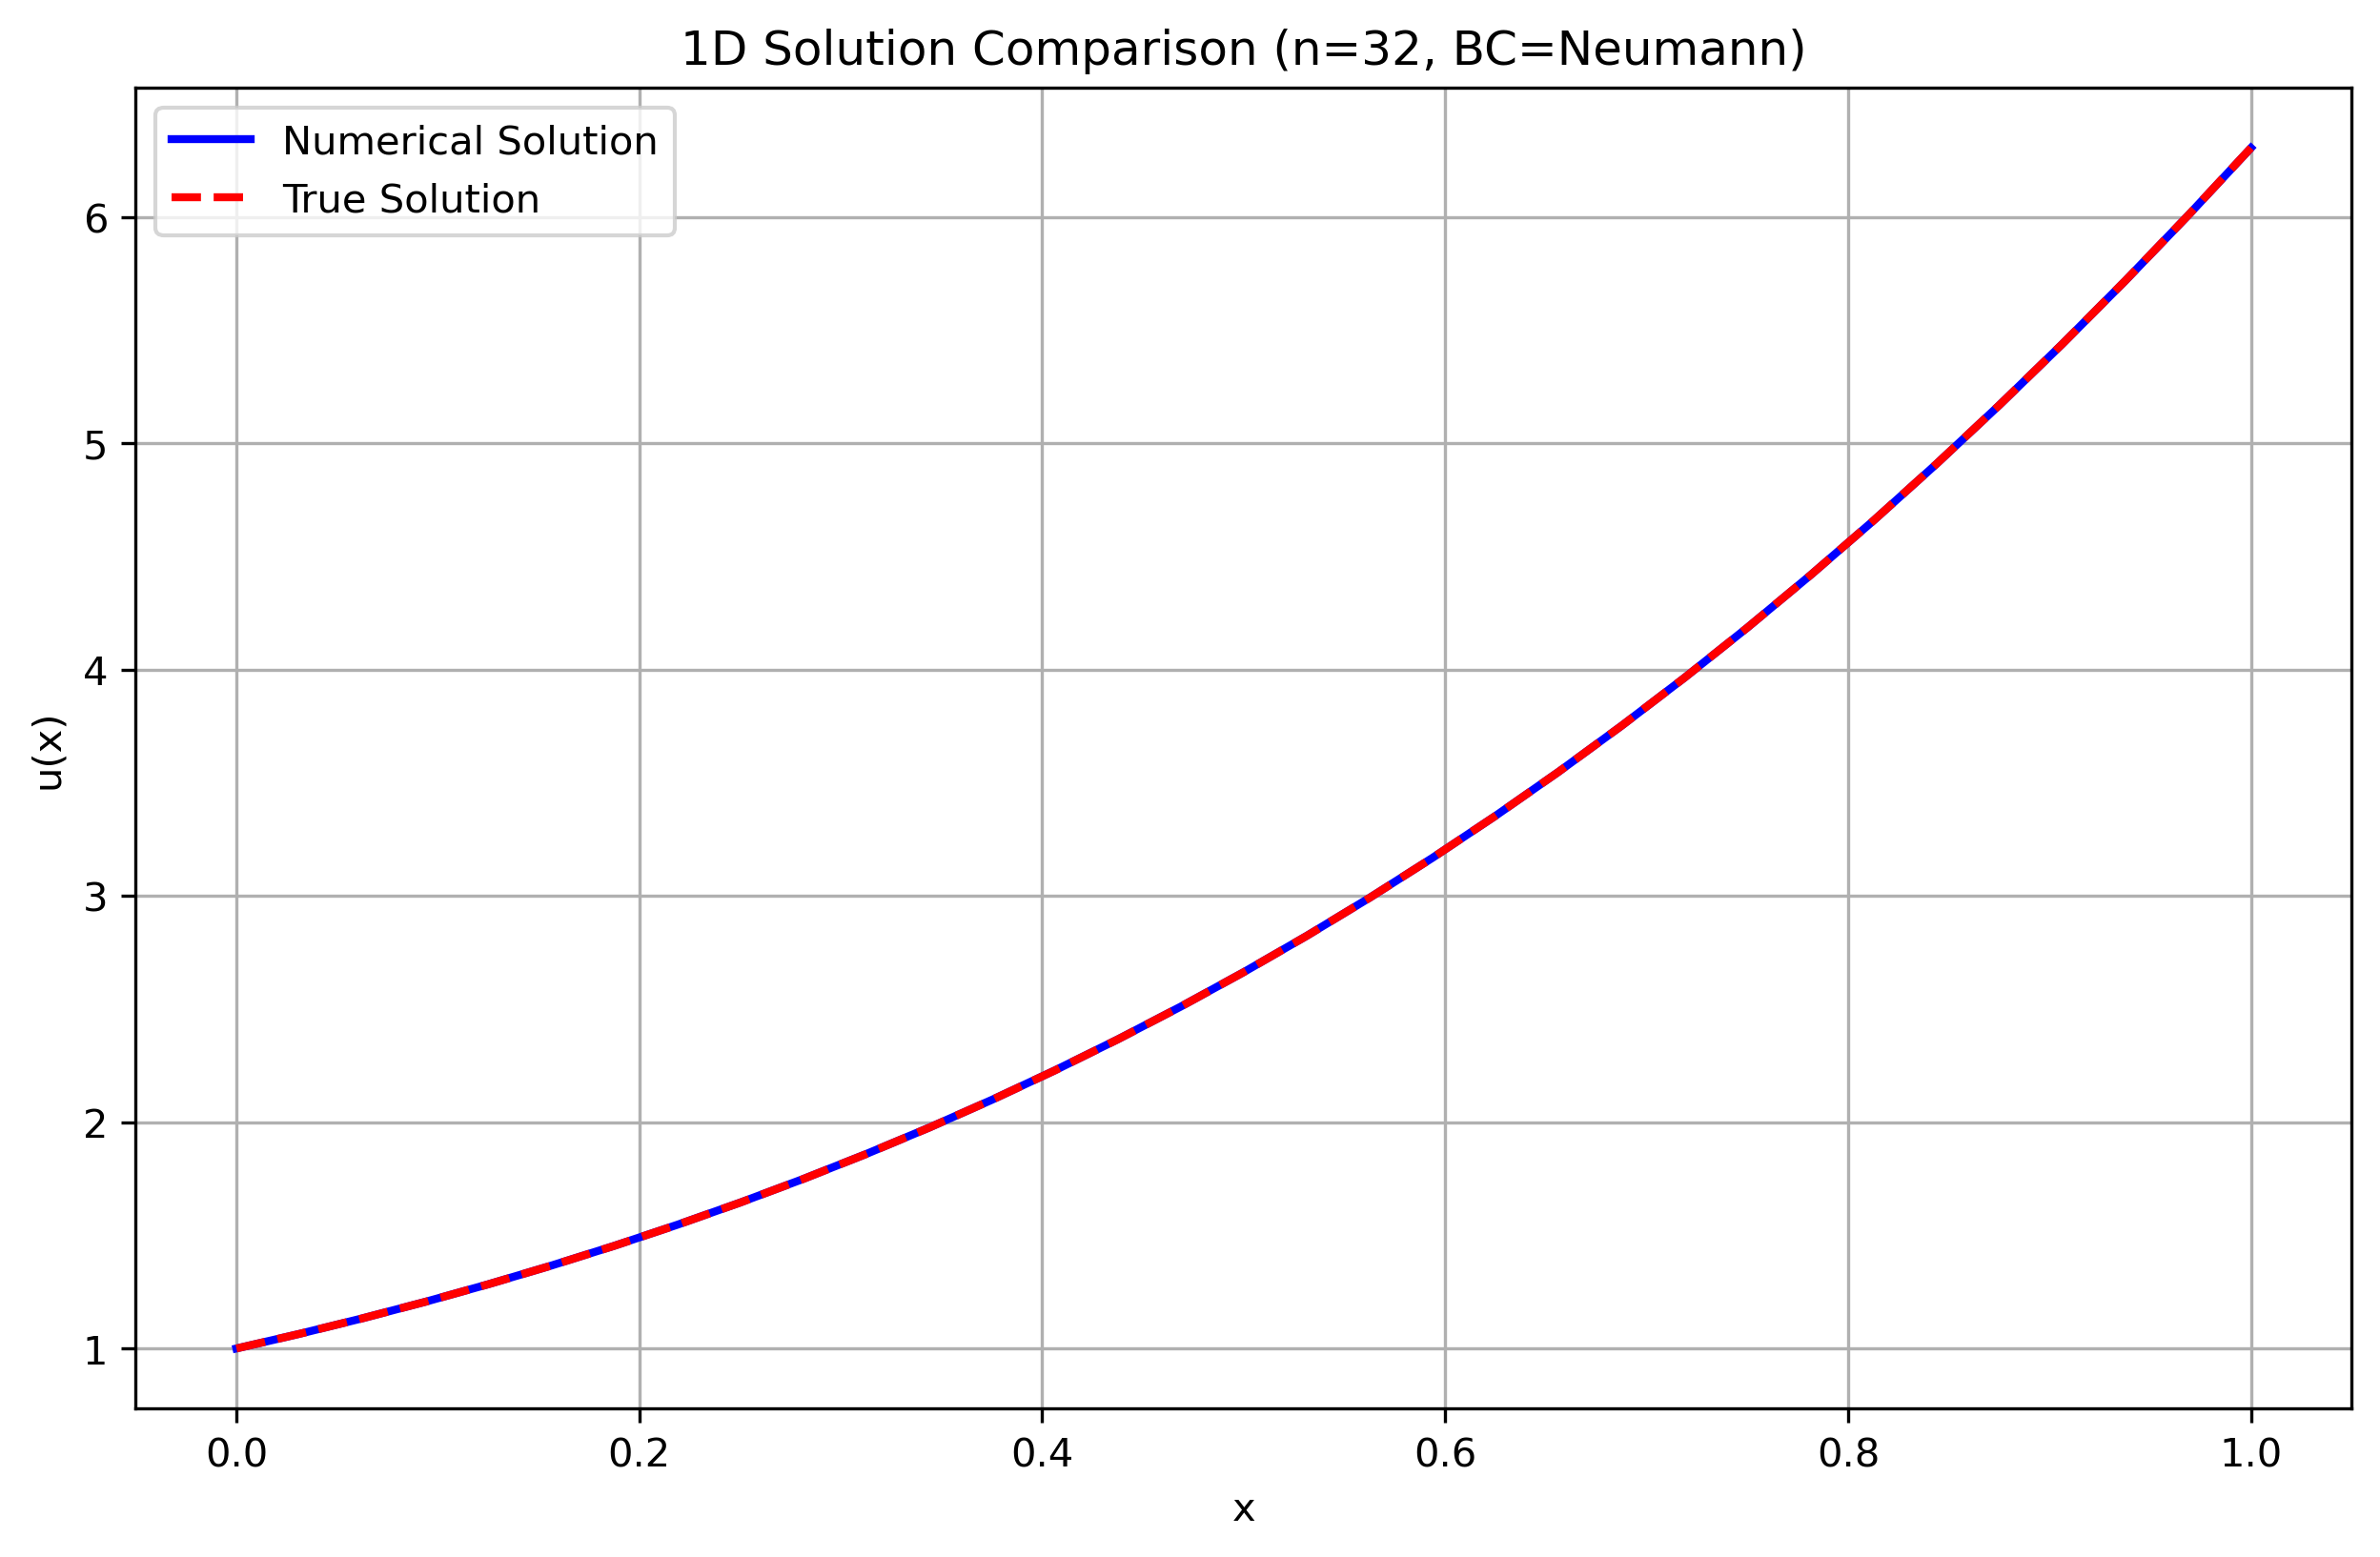
\includegraphics[width=\textwidth]{../plot/solution_dim1_n32_Neumann.png}
        \caption{$n=32, Neumann$}
    \end{subfigure}
    \hfill
    \begin{subfigure}[b]{0.45\textwidth}
        \centering
        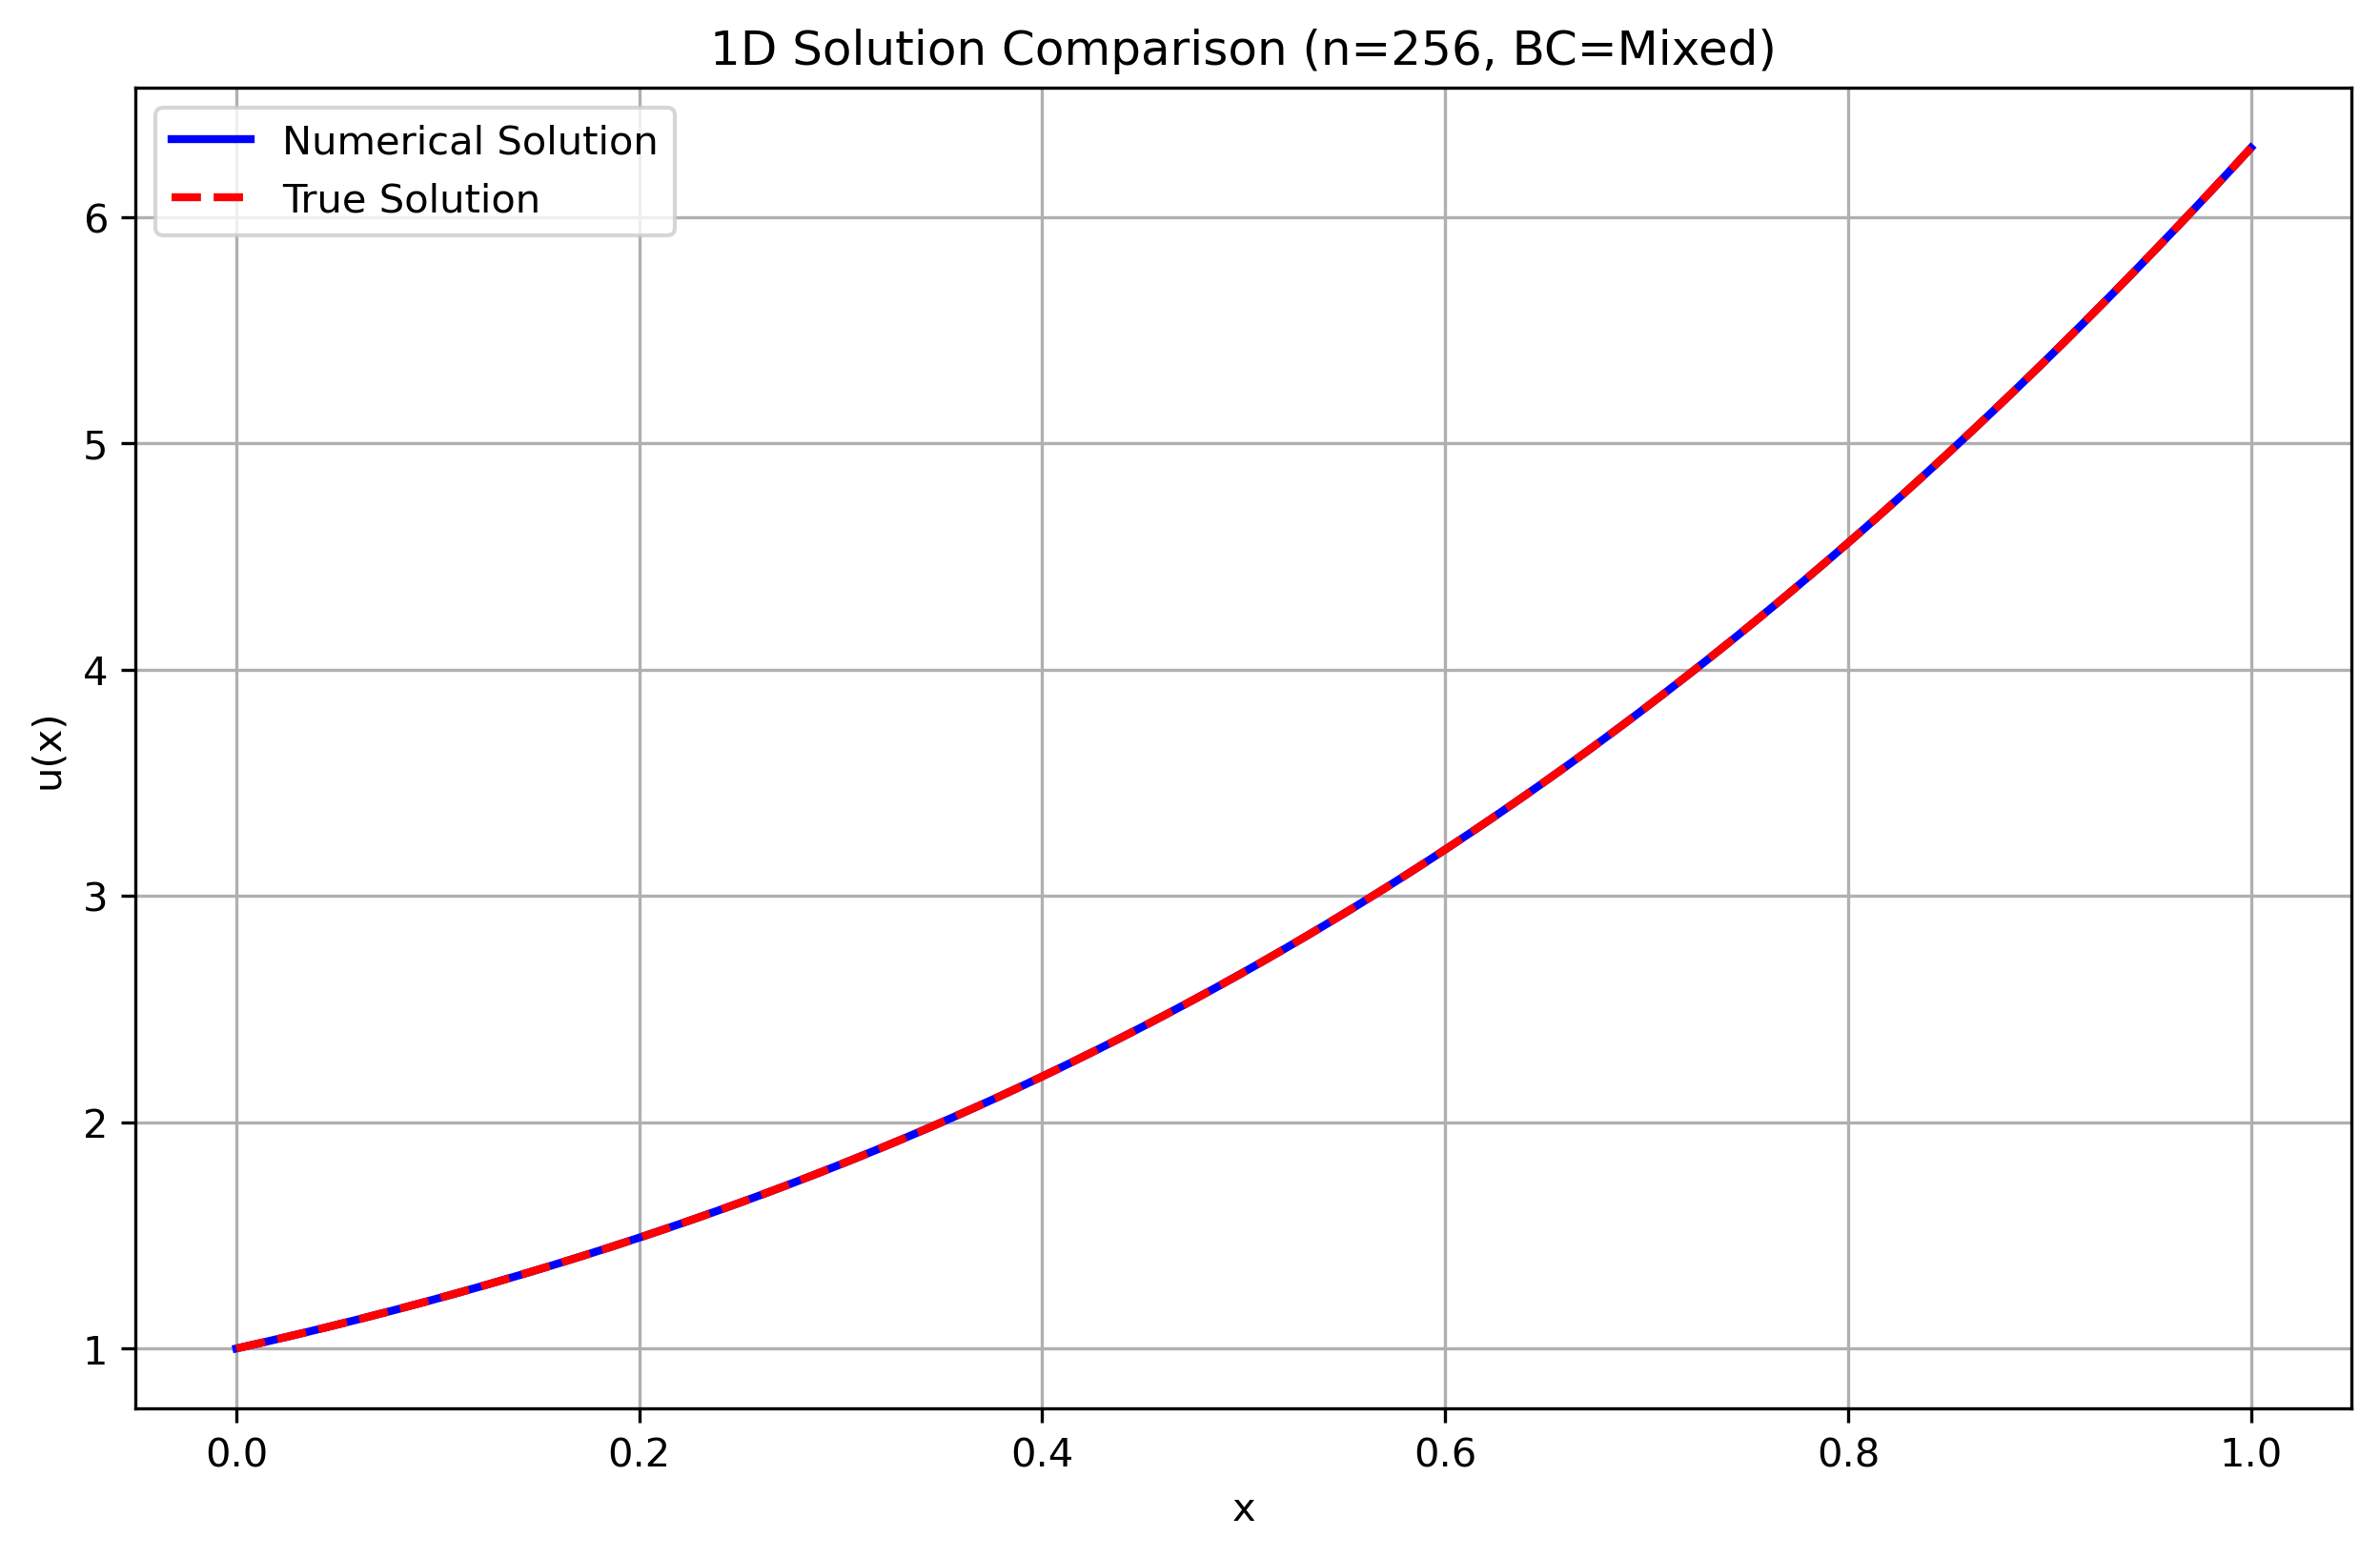
\includegraphics[width=\textwidth]{../plot/solution_dim1_n256_Mixed_DN.png}
        \caption{$n=256, Mixed$}
    \end{subfigure}
    \caption{一维情形}
\end{figure}

\begin{figure}[htbp]
    \centering
    \begin{subfigure}[b]{0.45\textwidth}
        \centering
        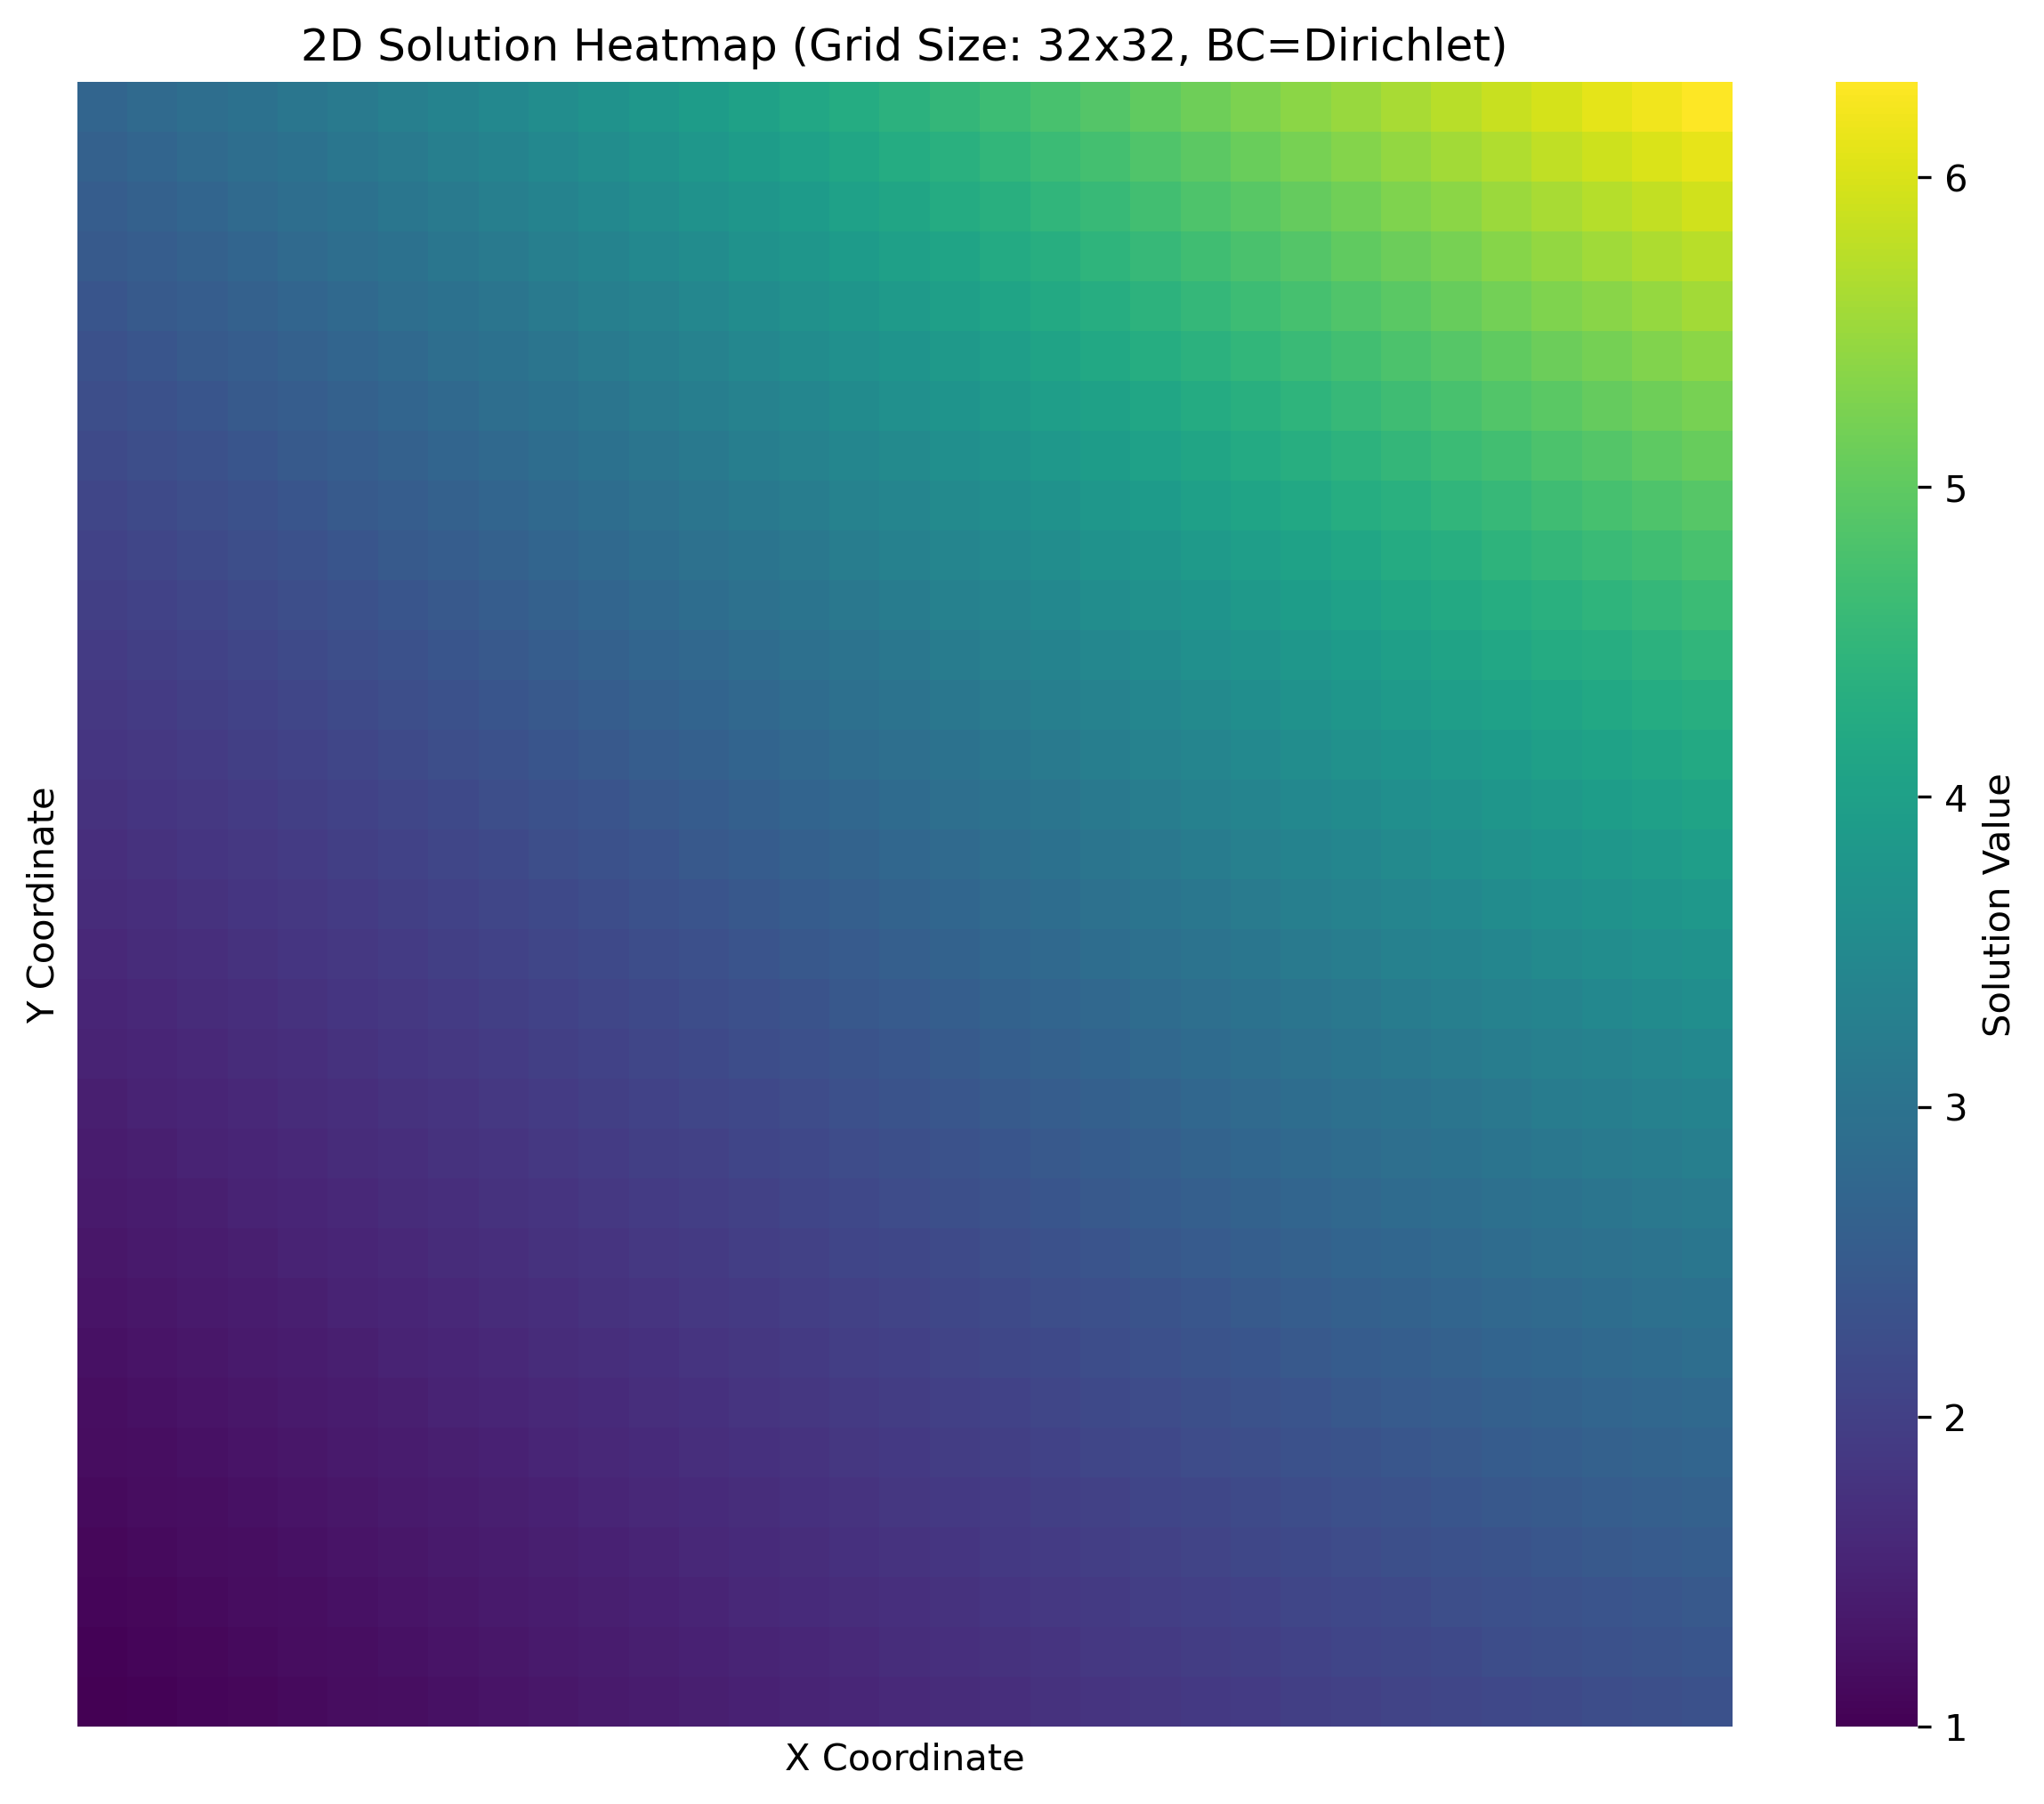
\includegraphics[width=\textwidth]{../plot/solution_dim2_n32_Dirichlet.png}
        \caption{$n=32, Dirichlet$}
    \end{subfigure}
    \hfill
    \begin{subfigure}[b]{0.45\textwidth}
        \centering
        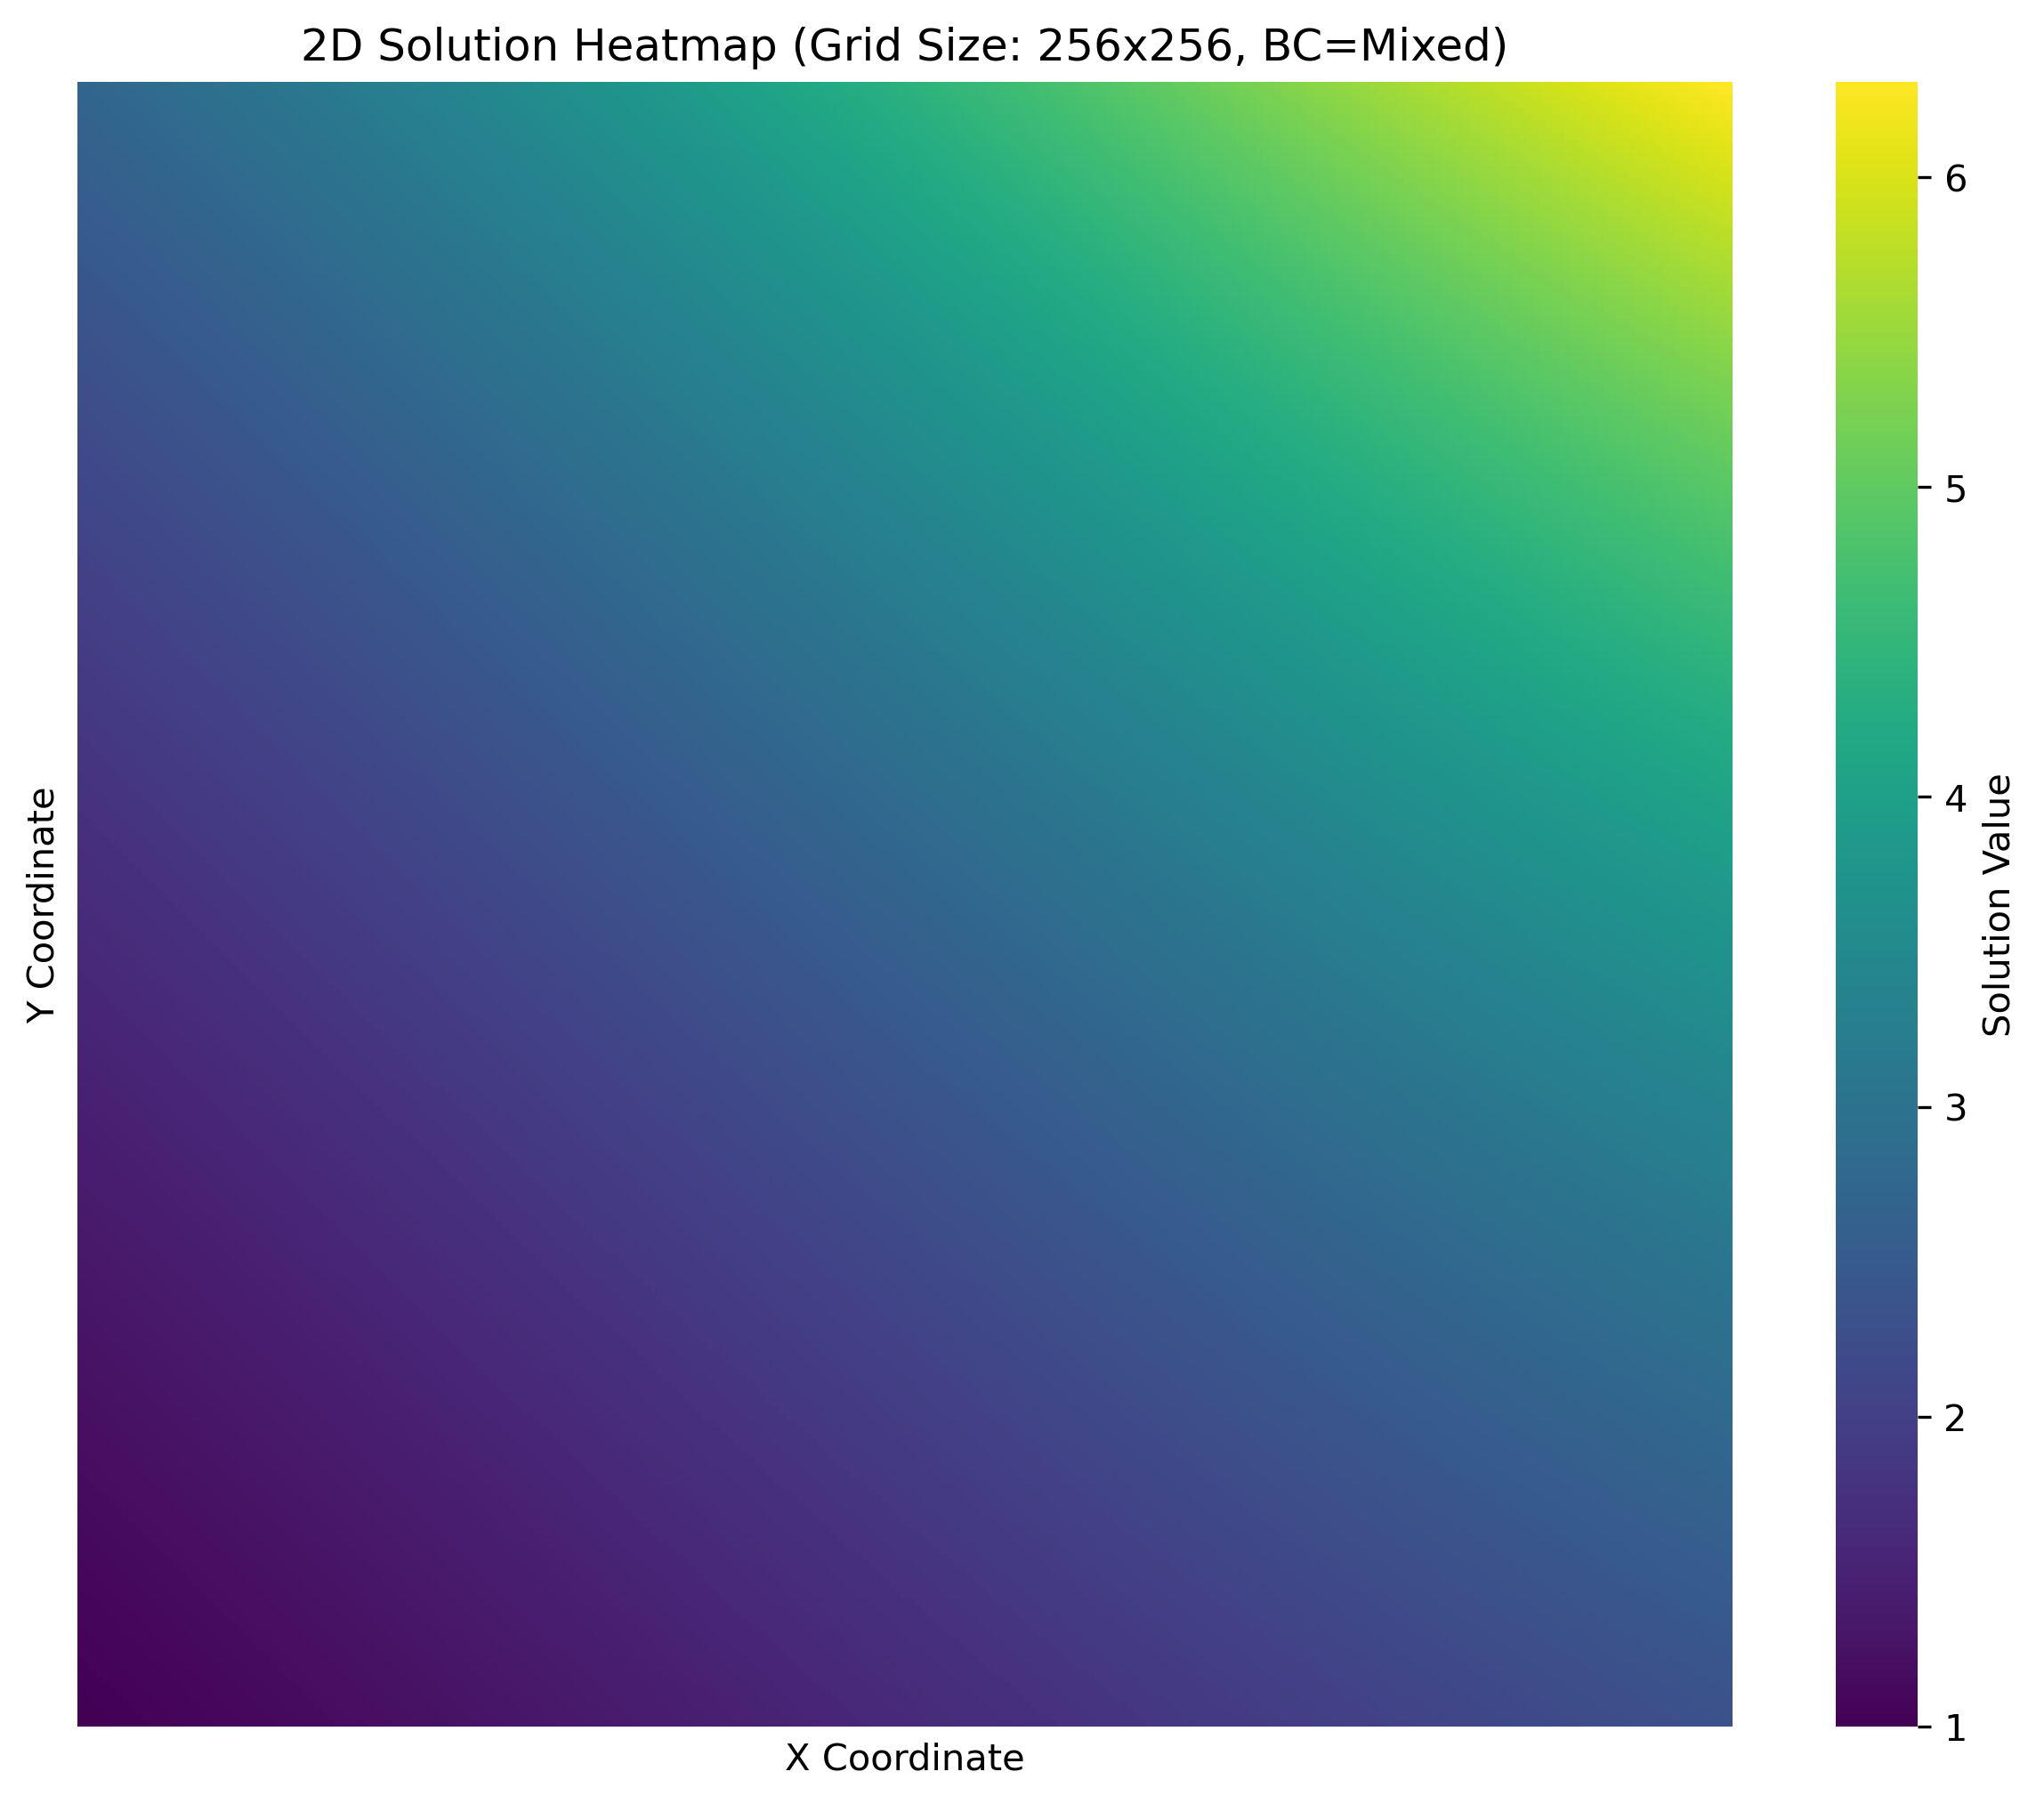
\includegraphics[width=\textwidth]{../plot/solution_dim2_n256_Mixed_DDNN.png}
        \caption{$n=256, Mixed-DDNN$}
    \end{subfigure}
    \caption{二维情形}
\end{figure}

\section{对不规则情形的单独说明}
本次作业也对下边界为
\[
{ (x, y) : y = \frac{1}{16}\sin(\pi x); \quad x \in [0, 1] }
\]
的情形做了实现，边界取为 Dirichlet 情形，采用扭曲网格法，即对格点做变换
\[
(i \cdot h, \, \text{IrF}(i \cdot h) + j \cdot h \cdot (1 - \text{IrF}(i \cdot h)) )
\]
其中 $\text{IrF} = \frac{1}{16}\sin(\pi x)$。

此时的离散与二维二次插值时相同，对 $P_0$ 点及其四个邻居格点 $P_1(i+1,j), P_2(i,j+1), P_3(i-1,j), P_4(i,j-1)$ 再加上其中一个角点（比如 $(i+1,j+1)$），进行泰勒展开，然后使得二阶项只剩下 $-\nabla^2 u(P_0)$，计算出对应点应附加的系数(在这里的系数计算是由普通的LU分解求得)。

同样为了对称的格式，我们对四个方向分别这样做，然后取平均得到我们最终的离散格式。


对这样求出的点，我对其绘制了散点热力图，可以看到与规则边界得到相同的解
\begin{figure}[htbp]
    \centering
    \begin{subfigure}[b]{0.45\textwidth}
        \centering
        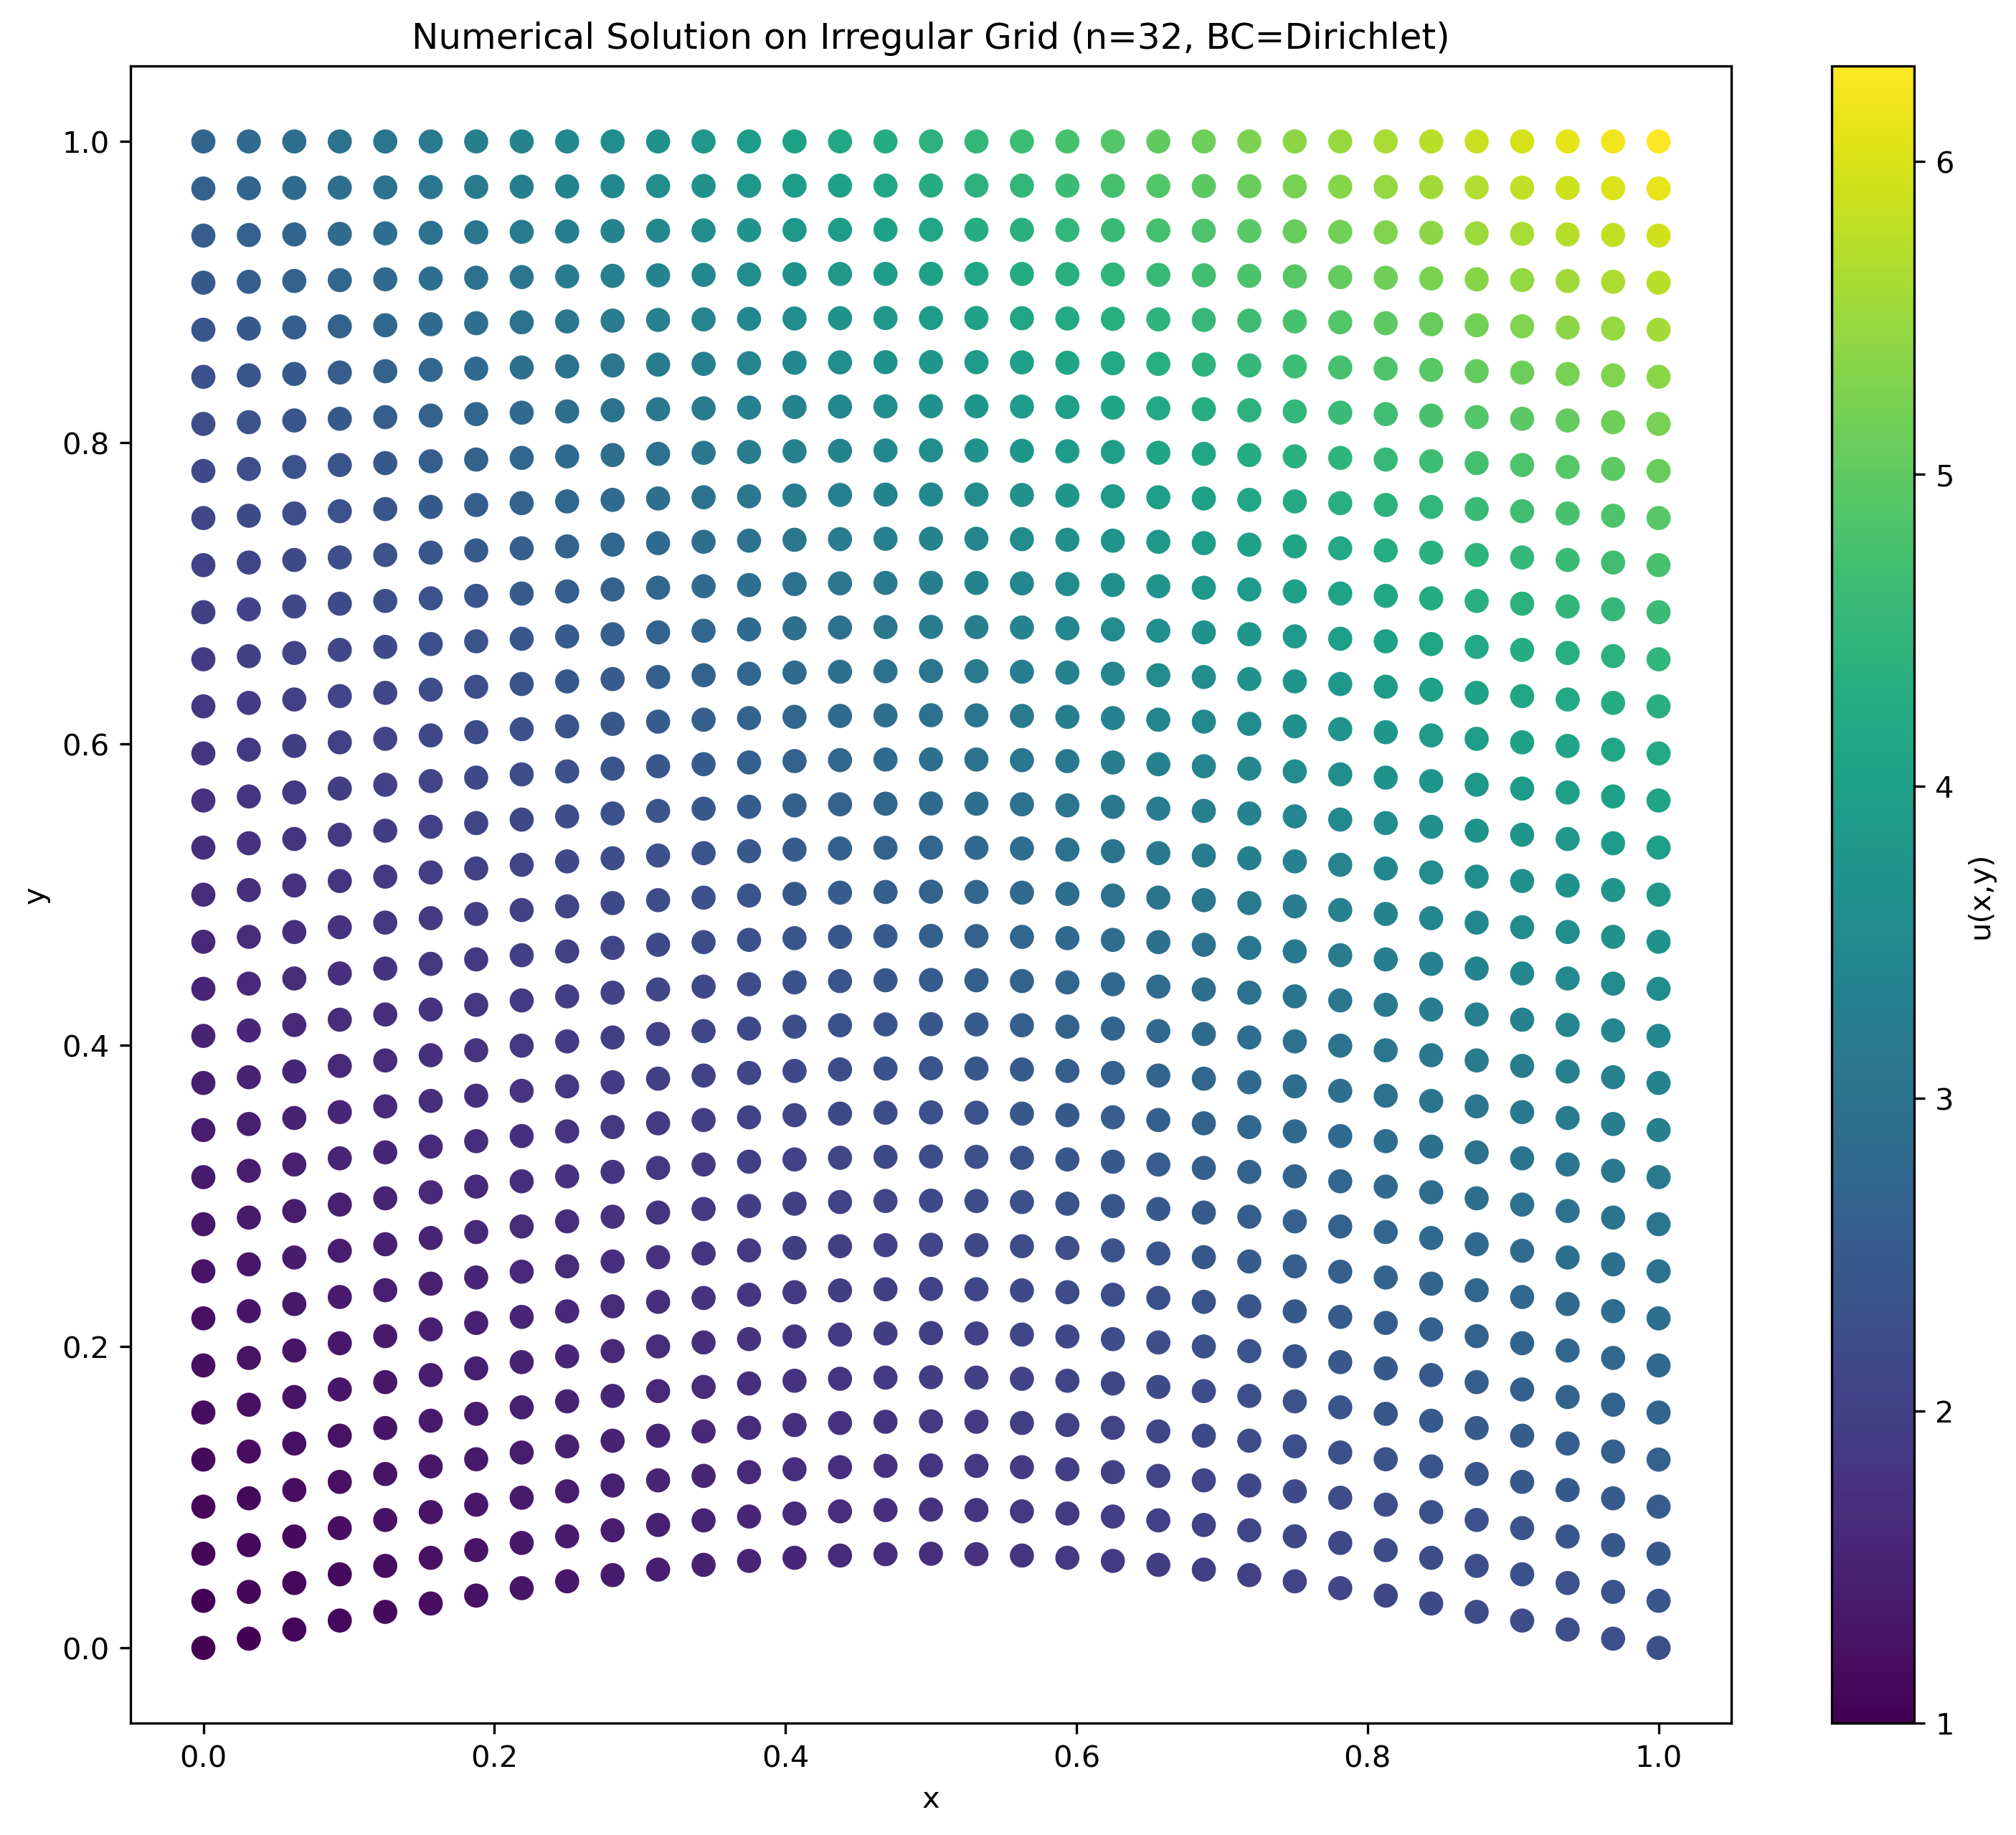
\includegraphics[width=\textwidth]{../plot/solution_dim2_n32_Dirichlet_irregular.png}
        \caption{$n=32$}
    \end{subfigure}
    \hfill
    \begin{subfigure}[b]{0.45\textwidth}
        \centering
        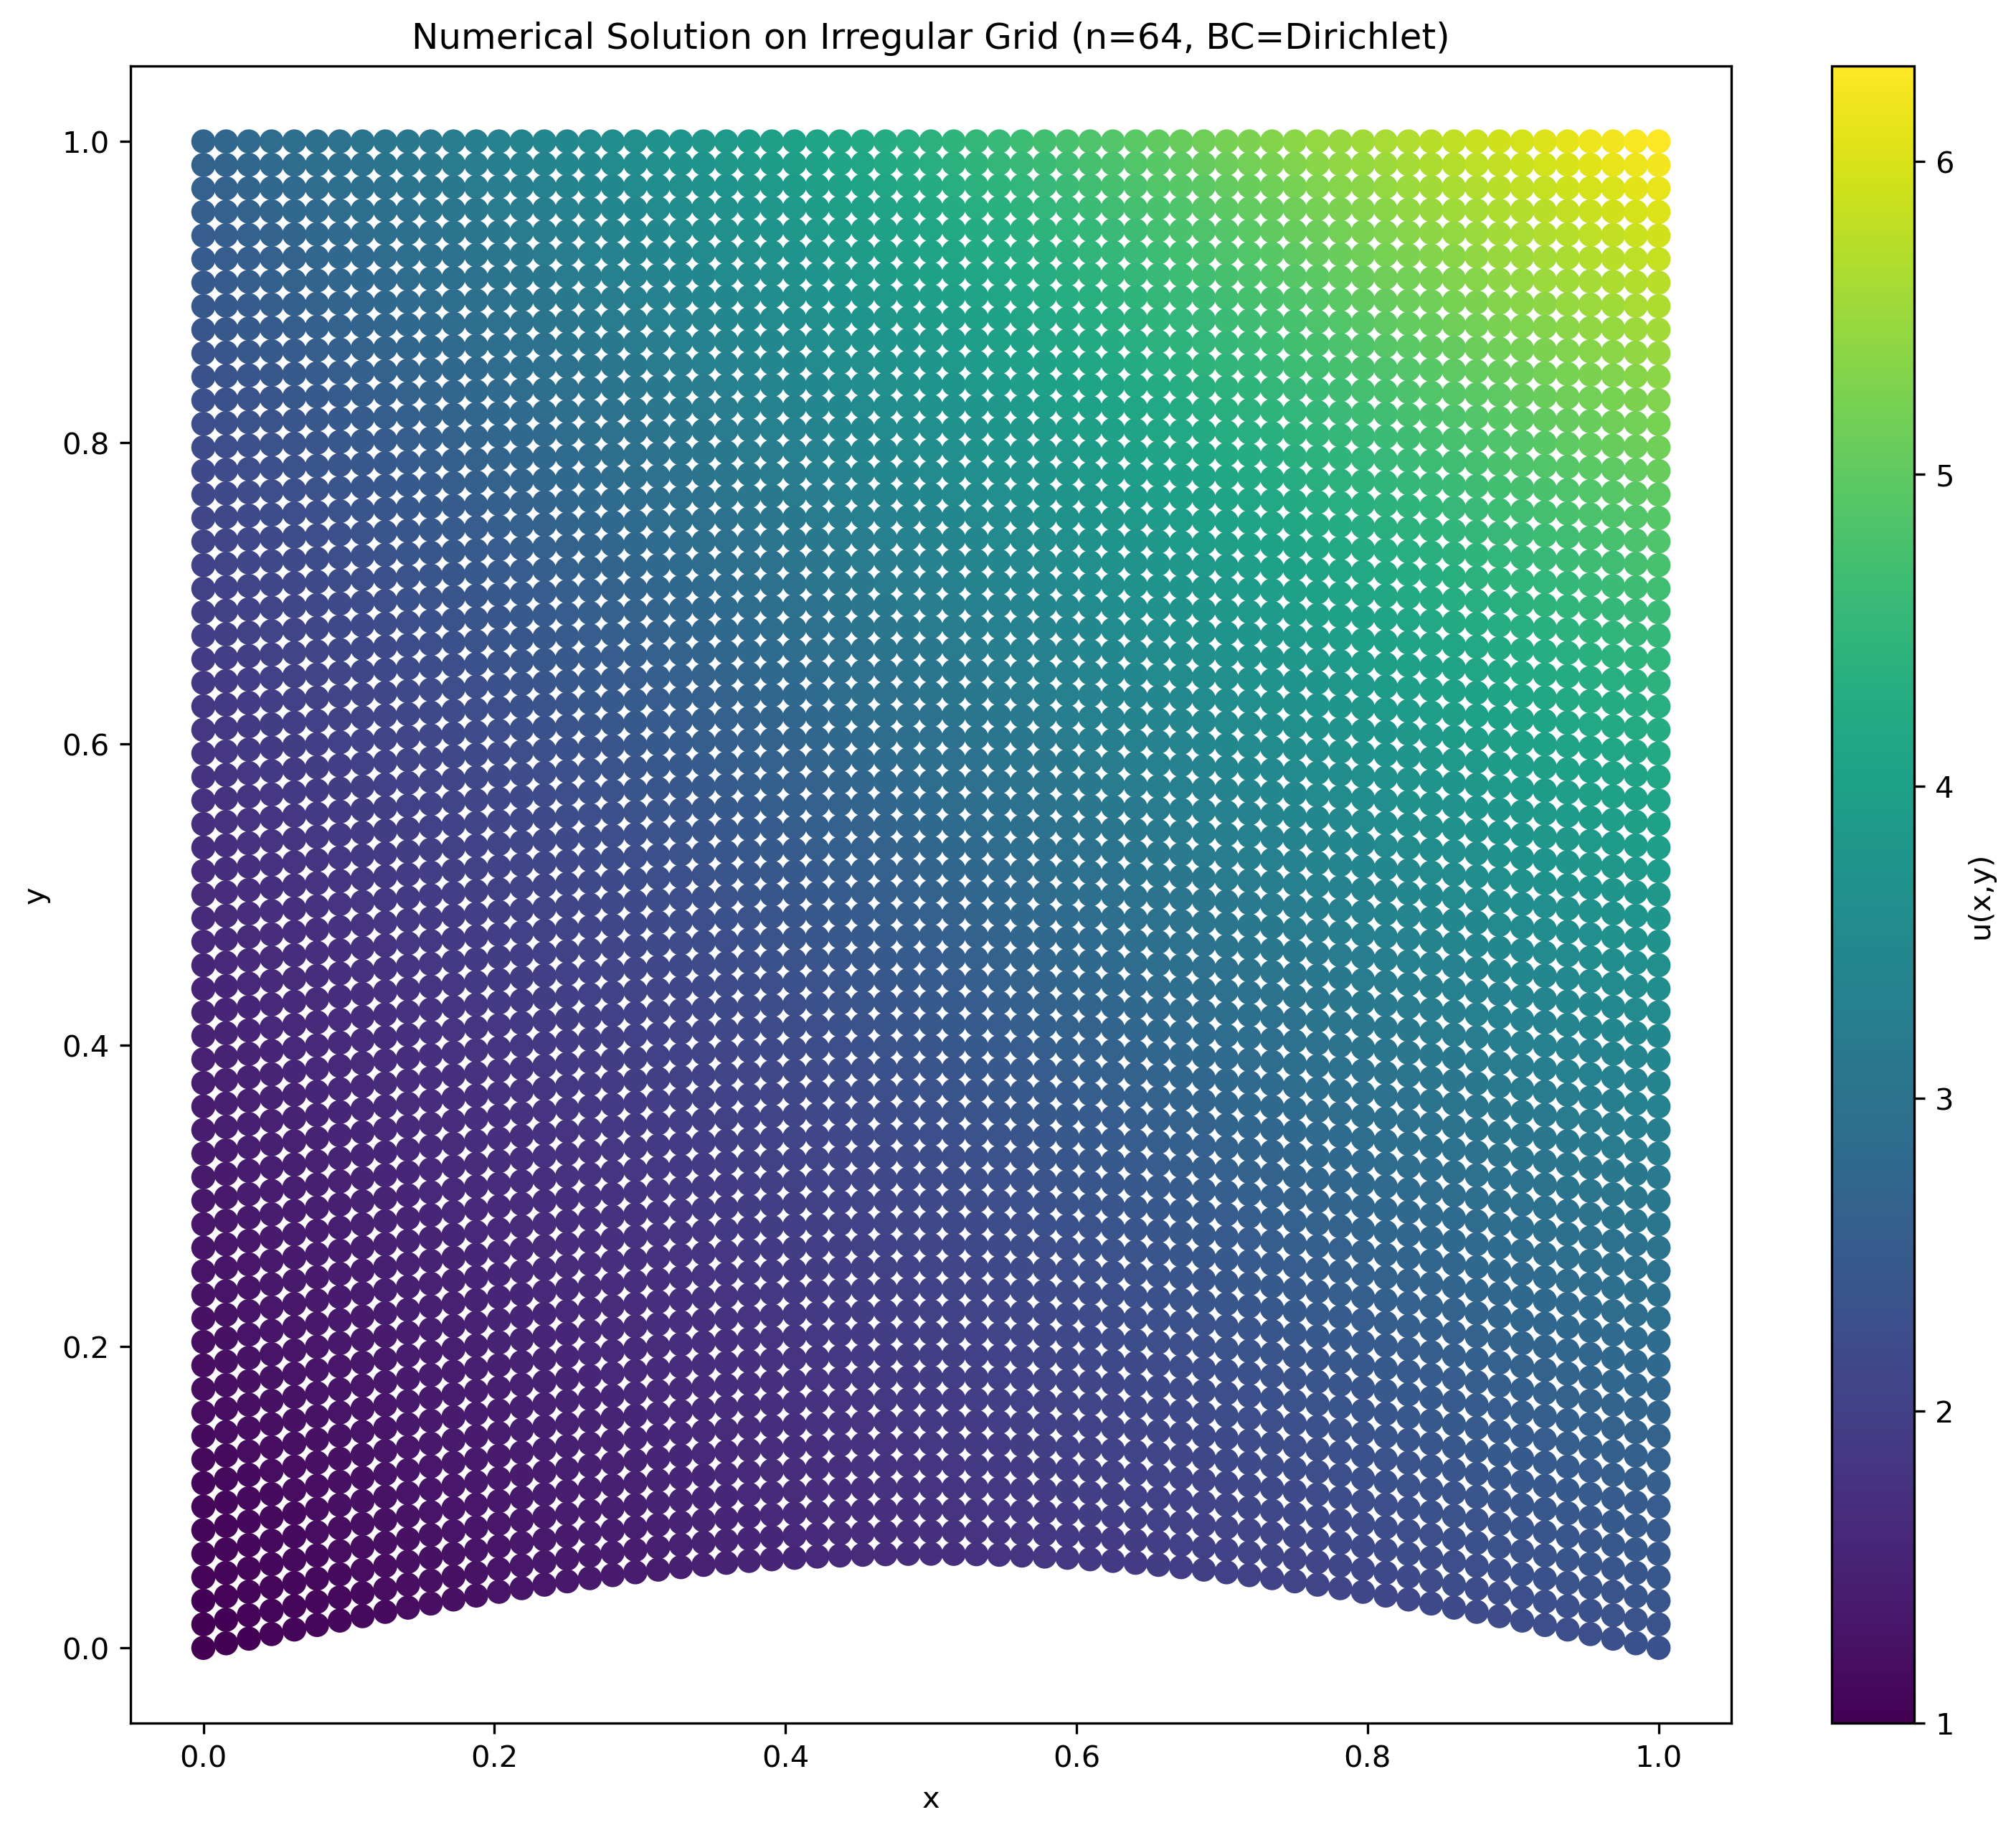
\includegraphics[width=\textwidth]{../plot/solution_dim2_n64_Dirichlet_irregular.png}
        \caption{$n=64$}
    \end{subfigure}
    \caption{可视化结果}
\end{figure}

\begin{figure}[htbp]
    \centering
    \begin{subfigure}[b]{0.45\textwidth}
        \centering
        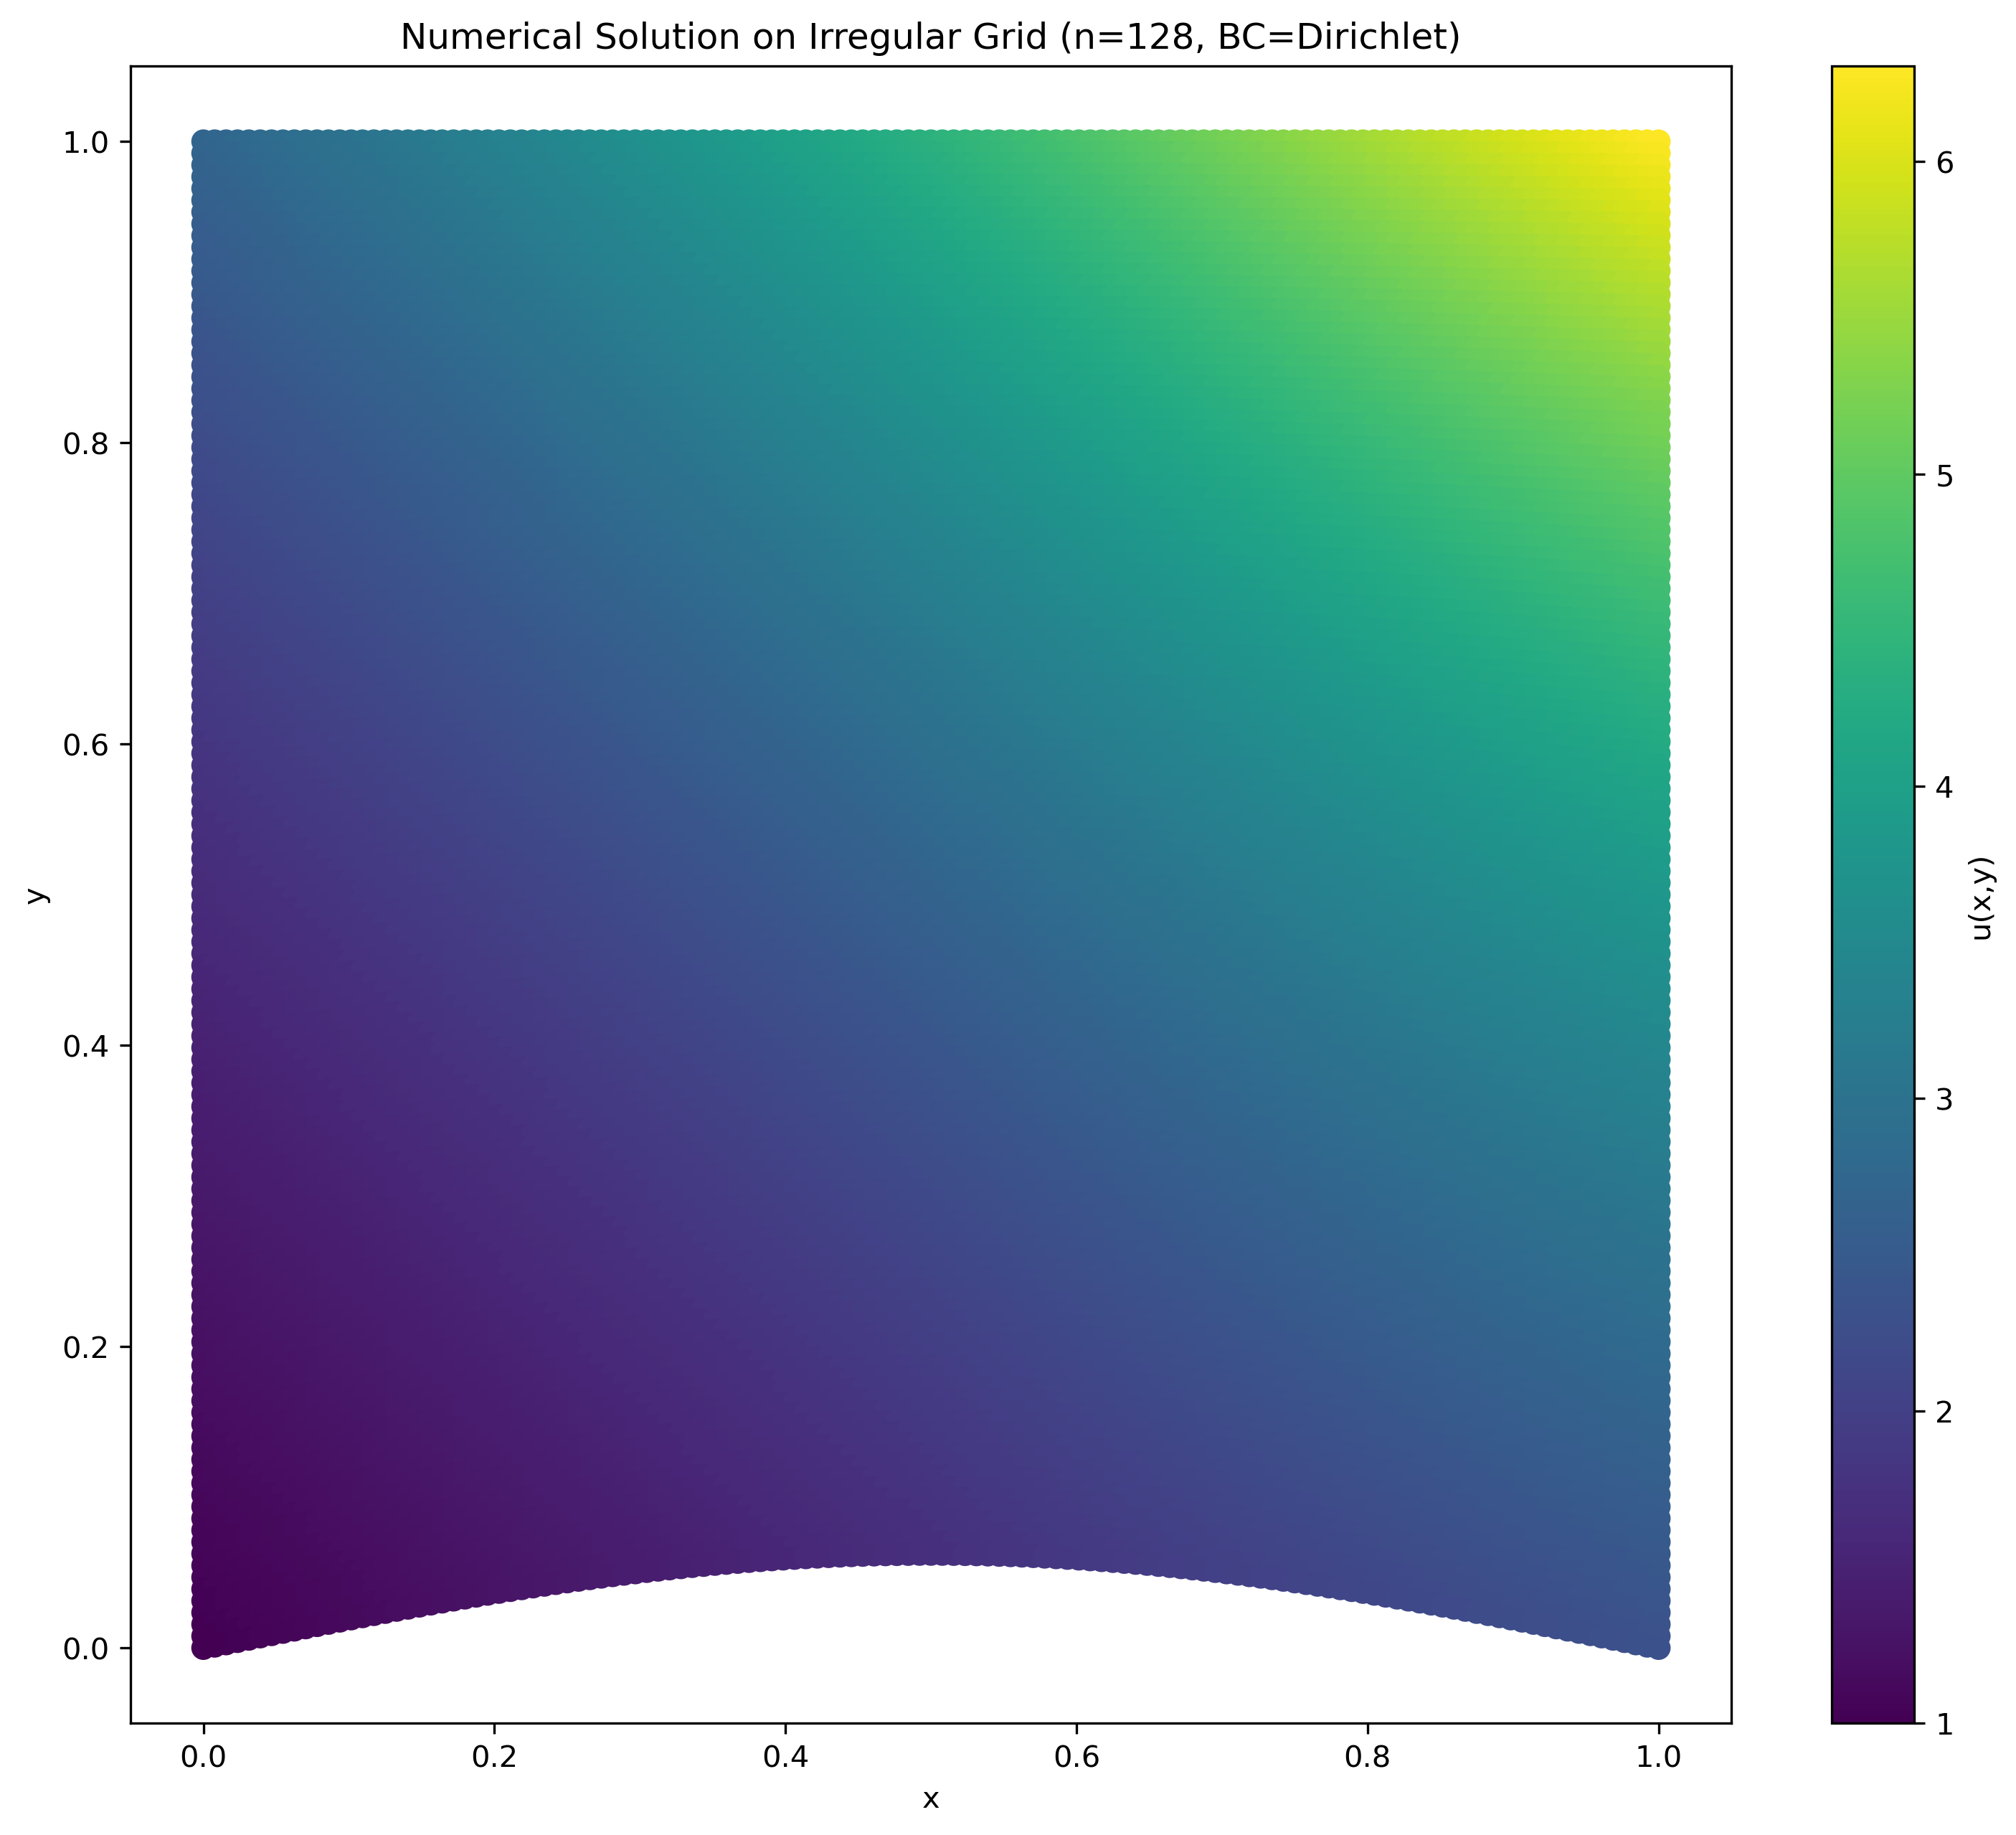
\includegraphics[width=\textwidth]{../plot/solution_dim2_n128_Dirichlet_irregular.png}
        \caption{$n=128$}
    \end{subfigure}
    \hfill
    \begin{subfigure}[b]{0.45\textwidth}
        \centering
        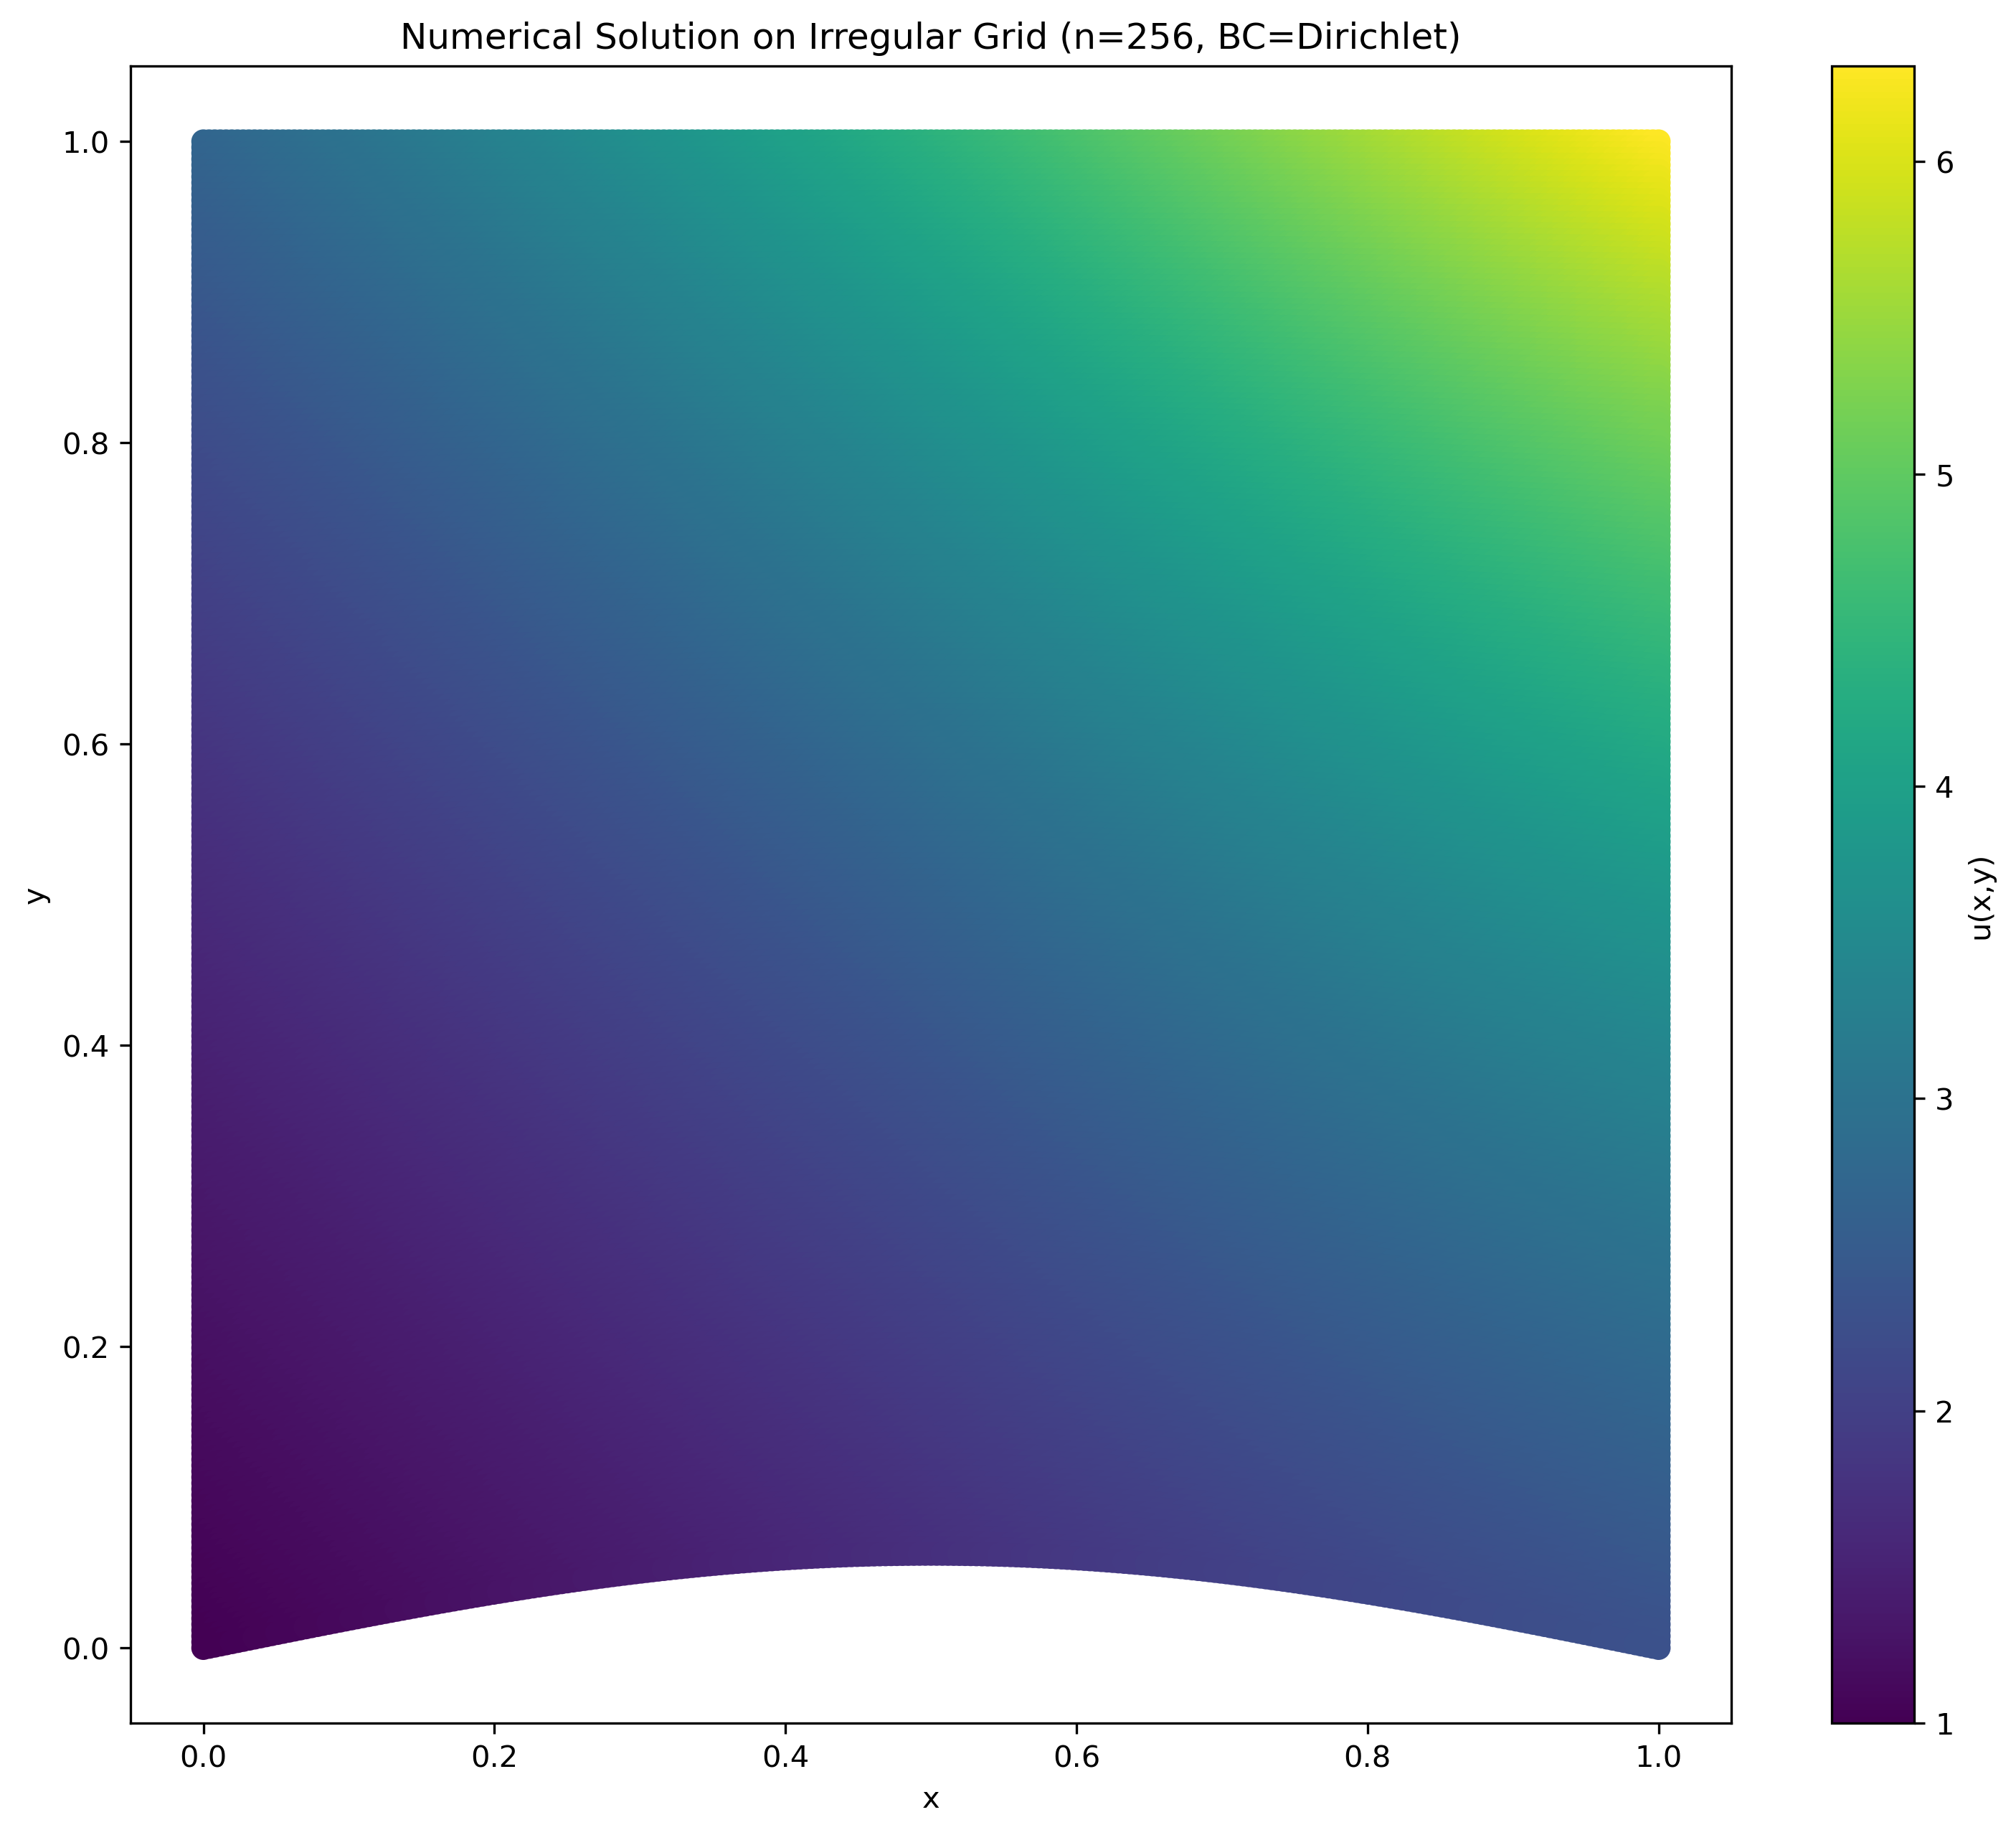
\includegraphics[width=\textwidth]{../plot/solution_dim2_n256_Dirichlet_irregular.png}
        \caption{$n=256$}
    \end{subfigure}
    \caption{可视化结果}
\end{figure}


\end{document}